\documentclass[xcolor=dvipsnames]{beamer}  

\mode<presentation>
{
  \usetheme{Singapore}
  % or ...
  \setbeamercovered{transparent}
  % or whatever (possibly just delete it)
}

\definecolor{pale}{RGB}{235, 235, 235}
\definecolor{pale2}{RGB}{175,238,238}
\definecolor{turquois4}{RGB}{0,134,139}
\definecolor{DarkOrange1}{RGB}{255,127,0}

%\setbeamercolor{block body}{fg=black, bg=green!10}
\setbeamercolor{block body}{fg=black, bg=pale}




%%%%%%%%%%%%%%%%%%%%%% start my preamble %%%%%%%%%%%%%%%%%%%%%%

% fonts
\usepackage{fontspec} 
\setmonofont{DejaVu Sans Mono}[Scale=MatchLowercase] % provides unicode characters 
\usefonttheme{professionalfonts}
\usepackage[T1]{fontenc}
\usepackage[mathscr]{euscript} 
\usepackage{stmaryrd} % St Mary's Road symbols font --- some extra symbols
\usepackage{bbm}


\renewcommand{\insertnavigation}[1]{}

\addtobeamertemplate{navigation symbols}{}{%
    \usebeamerfont{footline}%
    \usebeamercolor[fg]{footline}%
    \hspace{1em}%
    \insertframenumber/\inserttotalframenumber
    \vspace{0.5em}
}

\setbeamercolor{footline}{fg=blue}
\setbeamerfont{footline}{series=\bfseries}

%\setbeamertemplate{mini frames}{}

\usepackage{adjustbox}

\usepackage{graphicx}
\usepackage{amsmath, amssymb, amsthm, amsbsy}
\usepackage{mathtools}
\usepackage{fancyvrb}

\usepackage{hyperref}

% tikz
\usepackage{tikz}
\usepackage{tikz-cd}
\usetikzlibrary{positioning}
\usetikzlibrary{arrows}
\usetikzlibrary{calc}
\usetikzlibrary{intersections}
\usetikzlibrary{matrix}
\usetikzlibrary{decorations}
\usetikzlibrary{shapes, fit}
\usetikzlibrary{arrows.meta}
\usetikzlibrary{decorations.pathreplacing}  %for brac

\usepackage{pgf}
\usepackage{pgfplots}
\pgfplotsset{compat=1.7}


\usepackage{graphviz}

%\usepackage[usenames, dvipsnames]{color}


% nice inequalities
\renewcommand{\leq}{\leqslant}
\renewcommand{\geq}{\geqslant}


\setlength{\parskip}{1.5ex plus0.5ex minus0.5ex}
\setlength{\jot}{12pt} 

\usepackage[ruled, lined]{algorithm2e}
\SetKwBlock{Repeat}{repeat}{}  % repeat block has no end condition
\SetAlCapSkip{1.2em}


\newcommand{\emp}[1]{\textcolor{DarkOrange1}{\bf #1}}
\newcommand{\newtopic}[1]{\textcolor{Green}{\Large \bf #1}}
\newcommand{\navy}[1]{\textcolor{Blue}{\bf #1}}
\newcommand{\navymth}[1]{\textcolor{Blue}{#1}}
\newcommand{\red}[1]{\textcolor{red}{#1}}

% Minted
\definecolor{bg}{rgb}{0.95,0.95,0.95}
\usepackage{minted}
\usemintedstyle{friendly}
\newminted{python}{mathescape,frame=lines,framesep=4mm,bgcolor=bg}
\newminted{ipython}{mathescape,frame=lines,framesep=4mm,bgcolor=bg}
\newminted{julia}{mathescape,frame=lines,framesep=4mm,bgcolor=bg}
\newminted{c}{mathescape,frame=lines,framesep=4mm,bgcolor=bg}
\renewcommand{\theFancyVerbLine}{\sffamily
    \textcolor[rgb]{0.5,0.5,1.0}{\scriptsize {\arabic{FancyVerbLine}}}}


\newcommand{\Fact}{\textcolor{Brown}{\bf Fact. }}
\newcommand{\Facts}{\textcolor{Brown}{\bf Facts }}
\newcommand{\keya}{\textcolor{turquois4}{\bf Key Idea. }}
\newcommand{\Factnodot}{\textcolor{Brown}{\bf Fact }}
\newcommand{\Eg}{\textcolor{ForestGreen}{Example. }}
\newcommand{\Egs}{\textcolor{ForestGreen}{Examples. }}
\newcommand{\Ex}{{\bf Ex. }}


\newcommand{\CC}{\mathbbm C}
\newcommand{\EE}{\mathbbm E}
\newcommand{\FF}{\mathbbm F}
\newcommand{\RR}{\mathbbm R}
\newcommand{\KK}{\mathbbm K}
\newcommand{\MM}{\mathbbm M}
\newcommand{\NN}{\mathbbm N}
\newcommand{\PP}{\mathbbm P}
\newcommand{\TT}{\mathbbm T}
\newcommand{\QQ}{\mathbbm Q}
\newcommand{\WW}{\mathbbm W}
\newcommand{\VV}{\mathbbm V}
\newcommand{\ZZ}{\mathbbm Z}

\newcommand{\Asf}{\mathsf A}
\newcommand{\Esf}{\mathsf E}
\newcommand{\Fsf}{\mathsf F}
\newcommand{\Gsf}{\mathsf G}
\newcommand{\Msf}{\mathsf M}
\newcommand{\Lsf}{\mathsf L}
\newcommand{\Nsf}{\mathsf N}
\newcommand{\Psf}{\mathsf P}
\newcommand{\Qsf}{\mathsf Q}
\newcommand{\Ssf}{\mathsf S}
\newcommand{\Tsf}{\mathsf T}
\newcommand{\Xsf}{\mathsf X}
\newcommand{\Ysf}{\mathsf Y}
\newcommand{\Vsf}{\mathsf V}
\newcommand{\Wsf}{\mathsf W}
\newcommand{\Zsf}{\mathsf Z}

\newcommand{\aA}{\mathscr A}
\newcommand{\bB}{\mathscr B}
\newcommand{\cC}{\mathscr C}
\newcommand{\dD}{\mathscr D}
\newcommand{\eE}{\mathscr E}
\newcommand{\gG}{\mathscr G}
\newcommand{\hH}{\mathscr H}
\newcommand{\iI}{\mathscr I}
\newcommand{\fF}{\mathscr F}
\newcommand{\lL}{\mathscr L}
\newcommand{\pP}{\mathscr P}
\newcommand{\rR}{\mathscr R}
\newcommand{\sS}{\mathscr S}
\newcommand{\vV}{\mathscr V}
\newcommand{\wW}{\mathscr W}
\newcommand{\mM}{\mathscr M}
\newcommand{\oO}{\mathscr O}
\newcommand{\zZ}{\mathscr Z}

\newcommand{\bP}{\mathbf P} 
\newcommand{\bR}{\mathbf R}
\newcommand{\bQ}{\mathbf Q}


%%%%%% special symbols %%%%%%%%%%

% nice inequalities
\renewcommand{\leq}{\leqslant}
\renewcommand{\geq}{\geqslant}

% nice greek letters
\renewcommand{\phi}{\varphi}
\renewcommand{\epsilon}{\varepsilon}

% inner product
\providecommand{\inner}[1]{\left\langle{#1}\right\rangle}

% set of matrices
\newcommand{\matset}[2]{ \MM^{ #1 \times #2 } }

% stochastic dominance
\newcommand{\lefsd}{\preceq_{\textrm{F}}}
\newcommand{\lessd}{\preceq_{\textrm{S}}}

% argmax and min
\newcommand{\argmax}{\operatornamewithlimits{argmax}}
\newcommand{\argmin}{\operatornamewithlimits{argmin}}

% sets and logic
\newcommand{\st}{\ensuremath{\ \mathrm{s.t.}\ }}
\newcommand{\setntn}[2]{ \{ #1 : #2 \} }
\newcommand{\natset}[1]{[ #1 ]}

% some useful symbols
\newcommand{\given}{\, | \,}
\newcommand{\cf}[1]{ \lstinline|#1| }
\newcommand{\fore}{\therefore \quad}
\newcommand{\1}{\mathbbm 1}
\newcommand{\me}{\mathrm{e}}               % Euler's e
\newcommand*\diff{\mathop{}\!\mathrm{d}}   % d for integrals

% shortcuts
\newcommand{\la}{\langle}
\newcommand{\ra}{\rangle}

% relations
\newcommand{\eqdist}{\stackrel{d} {=} }
\newcommand{\iidsim}{\stackrel{\textrm{ {\sc iid }}} {\sim} }

% convergence
\newcommand{\tod}{\stackrel { d } {\to} }
\newcommand{\tow}{\stackrel { w } {\to} }
\newcommand{\toprob}{\stackrel { p } {\to} }
\newcommand{\toms}{\stackrel { ms } {\to} }


%%%%%%%%%%% operators %%%%%%%%%%%%

\DeclareMathOperator{\Fix}{fix}  % fixed point
\DeclareMathOperator{\Exp}{Exp}  % exponential draw
\DeclareMathOperator{\Lip}{Lip}
\DeclareMathOperator{\cl}{cl}
\DeclareMathOperator{\graph}{graph}
\DeclareMathOperator{\interior}{int}
\DeclareMathOperator{\Prob}{Prob}
\DeclareMathOperator{\determinant}{det}
\DeclareMathOperator{\trace}{trace}
\DeclareMathOperator{\sgn}{sgn}
\DeclareMathOperator{\Span}{span}
\DeclareMathOperator{\diag}{diag}
\DeclareMathOperator{\proj}{proj}
\DeclareMathOperator{\rank}{rank}
\DeclareMathOperator{\kernel}{null}
\DeclareMathOperator{\cov}{Cov}
\DeclareMathOperator{\corr}{Corr}
\DeclareMathOperator{\var}{Var}
\DeclareMathOperator{\mse}{mse}
\DeclareMathOperator{\se}{se}
\DeclareMathOperator{\range}{range}
\DeclareMathOperator{\dimension}{dim}





\hypersetup{
    linkcolor=Blue,
    colorlinks=true,
    filecolor=magenta,      % color of file links
    urlcolor=cyan           % color of external links
}


%\pgfdeclareimage[height=1.2cm]{university-logo}{../tuxswatter2}
%\logo{\pgfuseimage{university-logo}}

%\addtobeamertemplate{headline}{}
%{%
%\begin{flushright}
%\begin{tikzpicture}[remember picture,overlay]
%\node [left ]{\includegraphics[width=0.5cm]{../tuxswatter2.png}};
%\end{tikzpicture}
%\end{flushright}
%\vskip -0.1cm
%} 

 \date[\today]{}

\title{Dynamic Programming: Algorithms}

\author{John Stachurski}

\date{May 2024}



\begin{document}

\begin{frame}
  \titlepage
\end{frame}



\begin{frame}
    \frametitle{Topics}

    \begin{itemize}
        \item Value function iteration (VFI)
        \vspace{0.5em}
        \item Howard policy iteration (OPI)
        \vspace{0.5em}
        \item Optimistic policy iteration (HPI)
    \end{itemize}

        \vspace{0.5em}
        \vspace{0.5em}
        \vspace{0.5em}

    What convergence properties?
        \vspace{0.5em}

    How do they interact with parallelization? 

\end{frame}



\begin{frame}
    \frametitle{Example: optimal savings}
    
     Wealth evolves according to 

     \begin{equation*}
         w_{t+1} = Rw_t - c_t + y_t
     \end{equation*}


    \begin{itemize}
        \item $y$ is labor income
        \item $w$ is wealth
        \item $R$ is the gross rate of return on assets
    \end{itemize}

    \vspace{0.5em}
    \vspace{0.5em}
    Bellman equation:
    %
    \begin{equation*}
        v(w, y) = 
        \max_{0 \leq w' \leq w}
        \left\{
            u(Rw + y - w') 
             + \beta \sum_{y'} v(w', y') Q(y, y')
        \right\}
    \end{equation*}


\end{frame}



\begin{frame}

    A generalization:

    \begin{equation*}
            v(x)
            = \max_{a \in \Gamma(x)}
            \left\{
                r(x, a)
                + \beta
                \sum_{x' \in \Xsf} v(x') P(x, a, x')
            \right\}
    \end{equation*}
    %
    \vspace{0.5em}
    \vspace{0.5em}

    \begin{itemize}
        \item $x \in \Xsf$ is the \navy{state}
        \item $a \in \Asf$ is the \navy{action}
        \item $\Gamma(x) =$ actions available in state $x$
    \end{itemize}


\end{frame}






\begin{frame}
    \frametitle{Policies}

    
    A \navy{feasible policy} is a map $\sigma$ from $\Xsf$ to $\Asf$ such that
    %
    \begin{equation*}
            \sigma(x) \in \Gamma(x) \text{ for all } x \in \Xsf
    \end{equation*}
    %

    \begin{itemize}
        \item respond to $X_t$ with action $A_t = \sigma(X_t)$ at 
        \underline{all} $t \geq 0$
    \end{itemize}

    \vspace{0.5em}
    \vspace{0.5em}
    \vspace{0.5em}

    Let 
    %
    \begin{center}
            $\Sigma = $ the set of all feasible policies
    \end{center}




\end{frame}





\begin{frame}

     Let $v_\sigma(x) =$ lifetime value of policy $\sigma$, starting from $x$

    \vspace{0.5em}
    The function $v_\sigma$ satisfies
    
    \begin{equation*}
        v_\sigma(x) = r(x, \sigma(x)) + \beta \sum_{x'} v_\sigma(x')P(x, \sigma(x), x')
    \end{equation*}
    %

    Letting
    %
    \begin{itemize}
        \item $P_\sigma(x, x') = P(x, \sigma(x), x') =$ Markov dynamics given
            $\sigma$ and
        \vspace{0.5em}
        \item $r_\sigma(x) = r(x, \sigma(x)) = $ rewards at $x$ given $\sigma$
    \end{itemize}

    we can write this as the vector equation

    \begin{equation*}
        v_\sigma = r_\sigma + \beta P_\sigma v_\sigma
    \end{equation*}


\end{frame}

\begin{frame}
    
    How to solve
    %
    \begin{equation*}
        v_\sigma = r_\sigma + \beta P_\sigma v_\sigma
    \end{equation*}
    %
    for $v_\sigma$?

        \vspace{0.5em}
        \vspace{0.5em}
    Option 1: Use linear algebra to obtain
    %
    \begin{equation*}
        v_\sigma = (I - \beta P_\sigma)^{-1}  r_\sigma
    \end{equation*}

\end{frame}



\begin{frame}

   Option 2: Define the \navy{policy operator} corresponding to $\sigma$ is
    %
    \begin{equation*}
        (T_\sigma \, v)(x)
        =
            r(x, \sigma(x))
            + \beta
            \sum_{x' \in \Xsf} v(x') P(x, \sigma(x), x')
    \end{equation*}
    %



    \vspace{0.5em}
    In vector notation,
    %
    \begin{equation*}
        T_\sigma \, v 
        = r_\sigma + \beta P_\sigma v
    \end{equation*}
    %

    \vspace{0.5em}
    \vspace{0.5em}
    \vspace{0.5em}
    \vspace{0.5em}

    \Fact $T_\sigma$ is a contraction map on $\RR^n$

    \vspace{0.5em}
    Proof: Follows from
    %
    \begin{equation*}
        |T_\sigma \, v - T_\sigma \, w|
        \leq \beta |P_\sigma \, v - P_\sigma \, w|
    \end{equation*}

\end{frame}



\begin{frame}
    
    \Fact $v_\sigma$ is the unique fixed
    point of $T_\sigma$ in $\RR^n$ 

    \pause
    \vspace{0.5em}
    \vspace{0.5em}
    \underline{Proof}: Since $\beta < 1$, we have

    \begin{align*}
        v = T_\sigma \, v
        & \iff v = r_\sigma + \beta P_\sigma v
        \\
        & \iff v = (I - \beta P_\sigma)^{-1} \, r_\sigma 
        \\
        & \iff v = v_\sigma
    %
    \end{align*}

    \vspace{0.5em}
    Hence 
    $$v \text{ is a fixed point of } T_\sigma \; \iff \; v = v_\sigma $$

\end{frame}




\begin{frame}
    \frametitle{Greedy Policies}

    Fix $v \in \RR^n$ 
    
    \vspace{0.5em}
    \vspace{0.5em}
    \vspace{0.5em}
    A policy $\sigma$ is called
    \navy{$v$-greedy} if
    %
    \begin{equation*}
        \sigma(x)
        \in \argmax_{a \in \Gamma(x)}
        \left\{
            r(x, a)
            + \beta
            \sum_{x'} v(x') P(x, a, x')
        \right\}
    \end{equation*}
    %
    for all $x \in \Xsf$

    \vspace{0.5em}
    \vspace{0.5em}
    \vspace{0.5em}
    \Ex Prove: at least one $v$-greedy policy exists in $\Sigma$


\end{frame}


\begin{frame}
    
    \vspace{0.5em}
    The \navy{Bellman operator} is  defined by
    %
    \begin{equation*}
        (Tv)(x)
            = \max_{a \in \Gamma(x)}
            \left\{
                r(x, a)
                + \beta
                \sum_{x' } v(x') P(x, a, x')
            \right\}
    \end{equation*}
    %

    \vspace{0.5em}
    \vspace{0.5em}
    \vspace{0.5em}

    By construction, 

    \begin{center}
        $Tv=v$ $\iff$ $v$  satisfies the Bellman equation
    \end{center}

\end{frame}


\begin{frame}
    \frametitle{Optimality}

    \vspace{0.5em}
    The \navy{value function} is defined by
    %
    \begin{equation*}
        v^*(x) := \max_{\sigma \in \Sigma} v_\sigma(x)
        \qquad (x \in \Xsf)
    \end{equation*}
    %

    \vspace{0.5em}
    \vspace{0.5em}
    A policy $\sigma \in \Sigma$ is called \navy{optimal} if
    %
    \begin{equation*}
        v_\sigma = v^*
    \end{equation*}

\end{frame}




\begin{frame}\label{slide:mdp_result}

    Standard theory (Bellman, Denardo, Blackwell)

        \vspace{0.5em}
        \vspace{0.5em}
    \begin{block}{}
        {\bf Theorem.} For the DP model described above,
        %
        \vspace{0.5em}
        \begin{enumerate}
            \item $v^*$ is the unique fixed point of $T$
                in $\RR^n$
            \vspace{0.5em}
            \vspace{0.5em}
            \item A feasible policy is optimal if and only it is
                $v^*$-greedy
            \vspace{0.5em}
            \vspace{0.5em}
            \item At least one optimal policy exists
        \end{enumerate}
        %
    \end{block}



\end{frame}


\begin{frame}
    \frametitle{Algorithms}


    %
    \begin{enumerate}
        \item Value function iteration (HPI)
        \vspace{0.5em}
        \item Howard policy iteration (HPI) 
        \vspace{0.5em}
        \item Optimistic policy iteration (OPI)
    \end{enumerate}


\end{frame}


\begin{frame}
    
{\small 
    \begin{algorithm}[H]
    \DontPrintSemicolon
    input $v_0 \in \RR^n$\;
    \vspace{0.3em}
    input $\tau$\;
    \vspace{0.3em}
    $\epsilon \leftarrow \tau + 1$ \;
    \vspace{0.3em}
    $k \leftarrow 0$ \;
    \vspace{0.3em}
    \While{$\epsilon > \tau $}
    {
        $v_{k+1} \leftarrow Tv_k$ \;
    \vspace{0.3em}
        $\epsilon \leftarrow \| v_k - v_{k+1} \|_\infty$ \;
    \vspace{0.3em}
        $k \leftarrow k + 1$ \;
    \vspace{0.3em}
    }
    \vspace{0.3em}
    Compute a $v_k$-greedy policy $\sigma$ \;
    \vspace{0.3em}
    \Return{$\sigma$}
    \vspace{0.3em}
    \caption{VFI for MDPs}
    \end{algorithm}
}

\end{frame}

\begin{frame}
    

    VFI is 
    %
    \begin{itemize}
        \vspace{0.5em}
        \item easy to understand
        \vspace{0.5em}
        \item easy to implement 
        \vspace{0.5em}
        \item globally convergent
    \end{itemize}

    \vspace{0.5em}
    \vspace{0.5em}
    \vspace{0.5em}
    \vspace{0.5em}
    But the convergence rate is only linear  

\end{frame}


\begin{frame}
    \frametitle{Howard Policy Iteration}

    \begin{figure}
       \begin{center}
           \scalebox{0.7}{
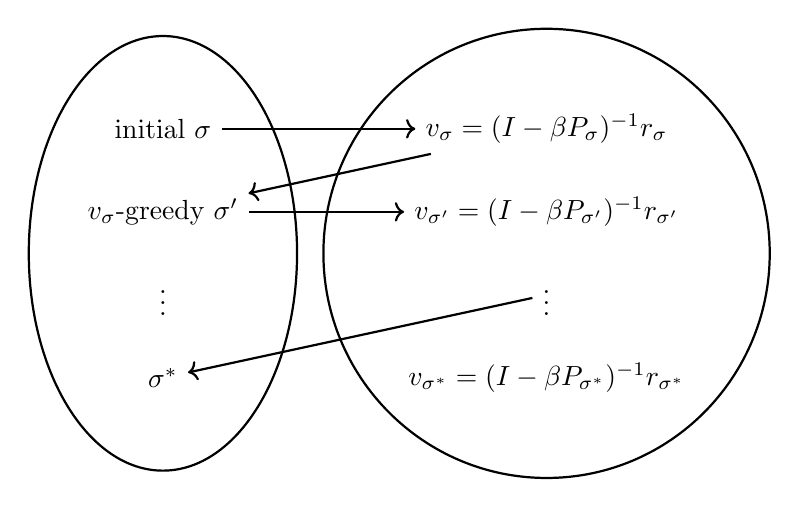
\begin{tikzpicture}[auto, thick, node distance=30pt]

\node (s) {initial $\sigma$};
\node (s1) [below of=s] {$v_{\sigma}$-greedy $\sigma'$};
\node (el1) [below of=s1] {$\vdots$};
\node (s2) [below of=el1] {$\sigma^*$};

\node (v) [right=70pt of s] {$v_{\sigma} = (I - \beta P_\sigma)^{-1} r_\sigma$};
\node (v1) [below of=v] {$v_{\sigma'} = (I - \beta P_{\sigma'})^{-1} r_{\sigma'}$};
\node (el2) [below of=v1] {$\vdots$};
\node (v2) [below of=el2] {$v_{\sigma^*} = (I - \beta P_{\sigma^*})^{-1} r_{\sigma^*}$};

\node[draw, ellipse, minimum width=50pt, fit=(s) (s1) (s2)](f1) {};
\node[draw, ellipse, minimum width=50pt, fit=(v) (v1) (v2)](f2) {};

\draw[->, bend left=0] (s) to (v);
\draw[->] (v) to (s1);
\draw[->] (s1) to (v1);
\draw[->] (el2) to (s2);

\end{tikzpicture}
}
        \vspace{1em}
       \end{center}
    \end{figure}

    Iterates between computing the value of a given policy
    and computing the greedy policy associated with that value

\end{frame}

\begin{frame}
        
    {\small
    \begin{algorithm}[H]
        \DontPrintSemicolon
        input $\sigma \in \Sigma$ \;
    \vspace{0.3em}
        $v_0 \leftarrow v_\sigma$ and $k \leftarrow 0$  \;
    \vspace{0.3em}
        \Repeat
        {
            $\sigma_k \leftarrow $ a $v_k$-greedy policy \;
    \vspace{0.3em}
            $v_{k+1} \leftarrow (I - \beta P_{\sigma_k} )^{-1} r_{\sigma_k}$ \;
    \vspace{0.3em}
            \lIf{$v_{k+1} = v_k$}{break} 
    \vspace{0.3em}
            $k \leftarrow k + 1$ \;
    \vspace{0.3em}
        }
        \Return{$\sigma_k$}
    \vspace{0.3em}
        \caption{Howard policy iteration for MDPs}
    \end{algorithm}
    }

\end{frame}

\begin{frame}
    
    \begin{block}{}
        {\bf Proposition.} 
            HPI returns an exact optimal policy in a finite number of steps
    \end{block}

    \vspace{0.5em}
    \vspace{0.5em}
    \vspace{0.5em}

    Also, rate of convergence is faster than VFI 

    \vspace{0.5em}
    \vspace{0.5em}

    In fact HPI $=$ gradient-based Newton iteration on $T$
    \vspace{0.5em}

    \begin{itemize}
        \item Implies a quadratic rate of convergence
        \vspace{0.5em}
        \item Details are in \url{https://dp.quantecon.org}
    \end{itemize}


\end{frame}

\begin{frame}
 
    \begin{figure} 
        \centering
        \scalebox{0.4}{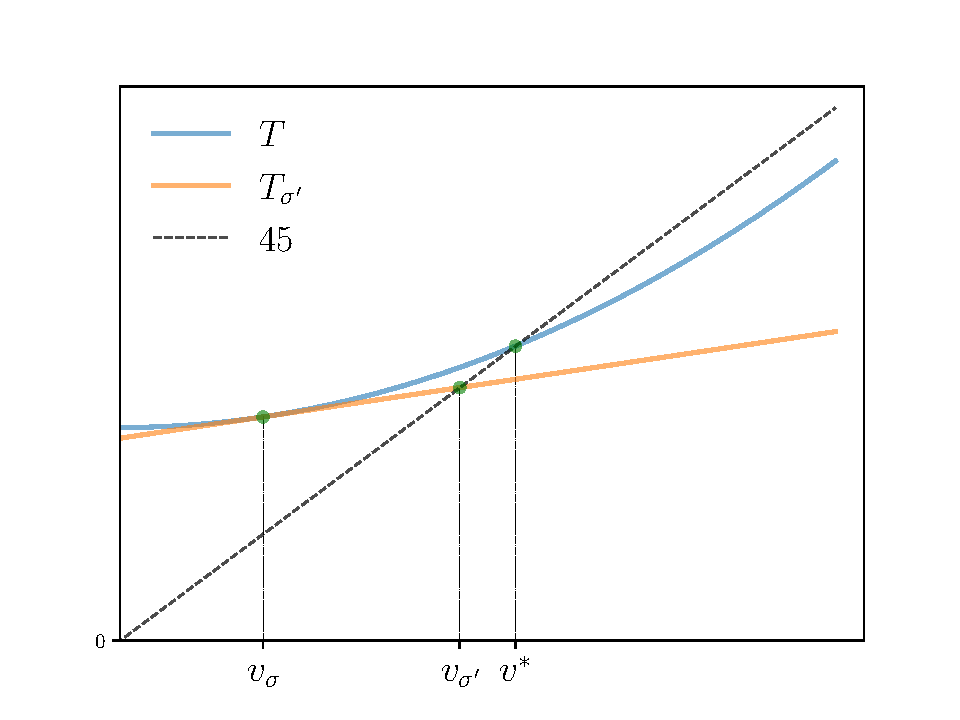
\includegraphics{figures/howard_newton_1.pdf}}
    \end{figure}
    %

    \begin{itemize}
        \item $\sigma'$ is $v_\sigma$-greedy if $T_{\sigma'} v_\sigma = T
            v_\sigma$
        \vspace{0.5em}
        \item $v_{\sigma'}$ is the fixed point of $T_{\sigma'}$
    \end{itemize}

\end{frame}


\begin{frame}
    \frametitle{Optimistic Policy Iteration}

    OPI is a ``convex combination'' of VFI and HPI

    \vspace{0.5em}
    Similar to HPI except that
    %
    \begin{itemize}
        \item HPI takes current $\sigma$ and obtains $v_\sigma$
    \vspace{0.5em}
        \item OPI takes current $\sigma$ and iterates $m$ times with $T_{\sigma}$
    \end{itemize}


    \vspace{0.5em}
    Recall that, for any $v \in \RR^n$, we have $T^m_{\sigma} v \to v_\sigma$ as $m \to \infty$

    \vspace{0.5em}
    \vspace{0.5em}
    Hence OPI replaces $v_\sigma$ with an approximation

\end{frame}


\begin{frame}
    
    {\small
    \begin{algorithm}[H]
        \DontPrintSemicolon
        input $v_0 \in \RR^n$\;
        \vspace{0.3em}
        input $\tau > 0$ and $m \in \NN$, a step size \;
        \vspace{0.3em}
        $k \leftarrow 0$ \;
        \vspace{0.3em}
        $\epsilon \leftarrow \tau + 1$ \;
        \vspace{0.3em}
        \While{$\epsilon > \tau $}
        {
            $\sigma_k \leftarrow $ a $v_k$-greedy policy \;
        \vspace{0.3em}
            $v_{k+1} \leftarrow T_{\sigma_k}^m v_k$  \;
        \vspace{0.3em}
            $\epsilon \leftarrow \| v_k - v_{k+1} \|_\infty$ \;
        \vspace{0.3em}
            $k \leftarrow k + 1$ \;
        }
        \vspace{0.3em}
        \Return{$\sigma_k$}
        \caption{Optimistic policy iteration for MDPs}
    \end{algorithm}
    }

\end{frame}


\begin{frame}

    \vspace{0.5em}
    \vspace{0.5em}
    \begin{block}{}
        {\bf Proposition.} For all values of $m$ we have $v_k \to v^*$
    \end{block}


\end{frame}

\begin{frame}



    It's easy to show that OPI $=$ VFI  when $m=1$


    On the other hand, $m$ is large, OPI is similar to HPI 


    \vspace{0.5em}
    \begin{itemize}
        \item because $\lim_{m \to \infty} T^m_{\sigma_k} v_k = v_{\sigma_k}$
    \end{itemize}


    \vspace{0.5em}
    \vspace{0.5em}
    \vspace{0.5em}
    Rules of thumb:

    \begin{itemize}
        \item parallelization favors HPI -- small number of expensive steps
        \vspace{0.5em}
        \item OFI is simple and dominates VFI for many values of $m$
        \vspace{0.5em}
        \item VFI works well when $\beta$ is small and optimization is cheap
    \end{itemize}


\end{frame}




\end{document}









